% Created by tikzDevice version 0.10.1 on 2017-10-23 14:01:33
% !TEX encoding = UTF-8 Unicode
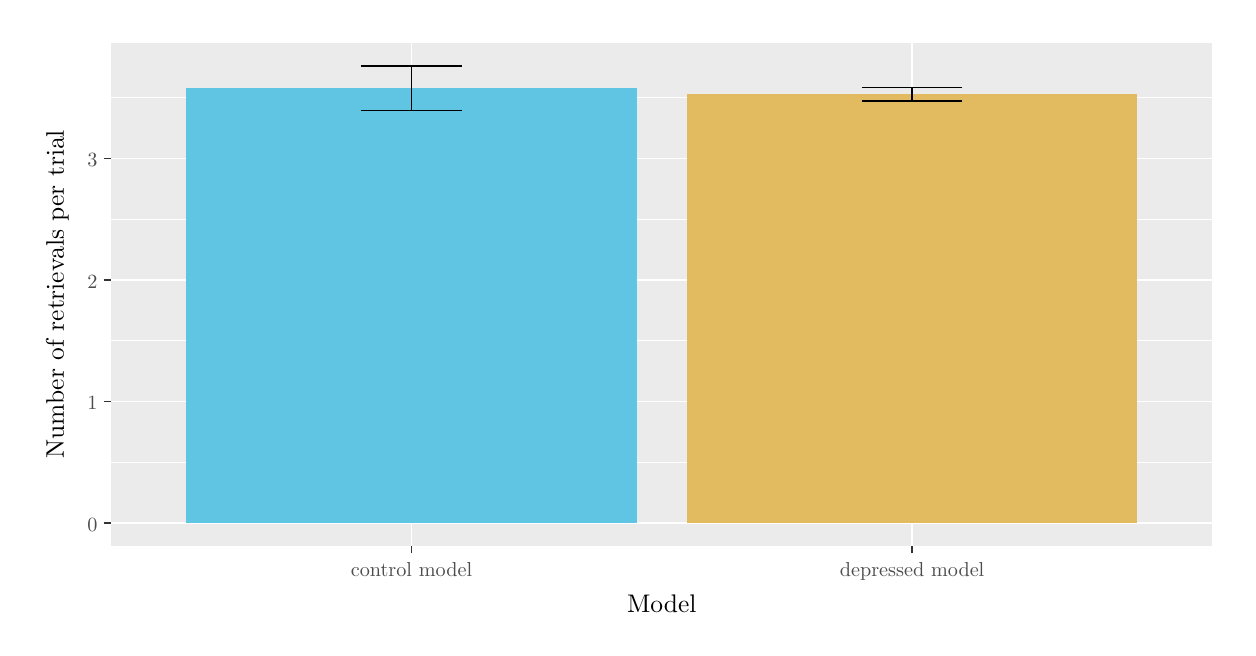
\begin{tikzpicture}[x=1pt,y=1pt]
\definecolor{fillColor}{RGB}{255,255,255}
\path[use as bounding box,fill=fillColor,fill opacity=0.00] (0,0) rectangle (433.62,216.81);
\begin{scope}
\path[clip] (  0.00,  0.00) rectangle (433.62,216.81);
\definecolor{drawColor}{RGB}{255,255,255}
\definecolor{fillColor}{RGB}{255,255,255}

\path[draw=drawColor,line width= 0.6pt,line join=round,line cap=round,fill=fillColor] (  0.00,  0.00) rectangle (433.62,216.81);
\end{scope}
\begin{scope}
\path[clip] ( 30.17, 29.59) rectangle (428.12,211.31);
\definecolor{fillColor}{gray}{0.92}

\path[fill=fillColor] ( 30.17, 29.59) rectangle (428.12,211.31);
\definecolor{drawColor}{RGB}{255,255,255}

\path[draw=drawColor,line width= 0.3pt,line join=round] ( 30.17, 59.79) --
	(428.12, 59.79);

\path[draw=drawColor,line width= 0.3pt,line join=round] ( 30.17,103.67) --
	(428.12,103.67);

\path[draw=drawColor,line width= 0.3pt,line join=round] ( 30.17,147.56) --
	(428.12,147.56);

\path[draw=drawColor,line width= 0.3pt,line join=round] ( 30.17,191.44) --
	(428.12,191.44);

\path[draw=drawColor,line width= 0.6pt,line join=round] ( 30.17, 37.85) --
	(428.12, 37.85);

\path[draw=drawColor,line width= 0.6pt,line join=round] ( 30.17, 81.73) --
	(428.12, 81.73);

\path[draw=drawColor,line width= 0.6pt,line join=round] ( 30.17,125.61) --
	(428.12,125.61);

\path[draw=drawColor,line width= 0.6pt,line join=round] ( 30.17,169.50) --
	(428.12,169.50);

\path[draw=drawColor,line width= 0.6pt,line join=round] (138.70, 29.59) --
	(138.70,211.31);

\path[draw=drawColor,line width= 0.6pt,line join=round] (319.59, 29.59) --
	(319.59,211.31);
\definecolor{fillColor}{RGB}{95,197,226}

\path[fill=fillColor] ( 57.30, 37.85) rectangle (220.10,194.98);
\definecolor{fillColor}{RGB}{226,186,95}

\path[fill=fillColor] (238.19, 37.85) rectangle (400.99,192.69);
\definecolor{drawColor}{RGB}{0,0,0}

\path[draw=drawColor,line width= 0.6pt,line join=round] (120.61,203.05) --
	(156.79,203.05);

\path[draw=drawColor,line width= 0.6pt,line join=round] (138.70,203.05) --
	(138.70,186.92);

\path[draw=drawColor,line width= 0.6pt,line join=round] (120.61,186.92) --
	(156.79,186.92);

\path[draw=drawColor,line width= 0.6pt,line join=round] (301.50,195.18) --
	(337.68,195.18);

\path[draw=drawColor,line width= 0.6pt,line join=round] (319.59,195.18) --
	(319.59,190.20);

\path[draw=drawColor,line width= 0.6pt,line join=round] (301.50,190.20) --
	(337.68,190.20);
\end{scope}
\begin{scope}
\path[clip] (  0.00,  0.00) rectangle (433.62,216.81);
\definecolor{drawColor}{gray}{0.30}

\node[text=drawColor,anchor=base east,inner sep=0pt, outer sep=0pt, scale=  0.73] at ( 25.22, 34.82) {0};

\node[text=drawColor,anchor=base east,inner sep=0pt, outer sep=0pt, scale=  0.73] at ( 25.22, 78.70) {1};

\node[text=drawColor,anchor=base east,inner sep=0pt, outer sep=0pt, scale=  0.73] at ( 25.22,122.58) {2};

\node[text=drawColor,anchor=base east,inner sep=0pt, outer sep=0pt, scale=  0.73] at ( 25.22,166.47) {3};
\end{scope}
\begin{scope}
\path[clip] (  0.00,  0.00) rectangle (433.62,216.81);
\definecolor{drawColor}{gray}{0.20}

\path[draw=drawColor,line width= 0.6pt,line join=round] ( 27.42, 37.85) --
	( 30.17, 37.85);

\path[draw=drawColor,line width= 0.6pt,line join=round] ( 27.42, 81.73) --
	( 30.17, 81.73);

\path[draw=drawColor,line width= 0.6pt,line join=round] ( 27.42,125.61) --
	( 30.17,125.61);

\path[draw=drawColor,line width= 0.6pt,line join=round] ( 27.42,169.50) --
	( 30.17,169.50);
\end{scope}
\begin{scope}
\path[clip] (  0.00,  0.00) rectangle (433.62,216.81);
\definecolor{drawColor}{gray}{0.20}

\path[draw=drawColor,line width= 0.6pt,line join=round] (138.70, 26.84) --
	(138.70, 29.59);

\path[draw=drawColor,line width= 0.6pt,line join=round] (319.59, 26.84) --
	(319.59, 29.59);
\end{scope}
\begin{scope}
\path[clip] (  0.00,  0.00) rectangle (433.62,216.81);
\definecolor{drawColor}{gray}{0.30}

\node[text=drawColor,anchor=base,inner sep=0pt, outer sep=0pt, scale=  0.73] at (138.70, 18.58) {control model};

\node[text=drawColor,anchor=base,inner sep=0pt, outer sep=0pt, scale=  0.73] at (319.59, 18.58) {depressed model};
\end{scope}
\begin{scope}
\path[clip] (  0.00,  0.00) rectangle (433.62,216.81);
\definecolor{drawColor}{RGB}{0,0,0}

\node[text=drawColor,anchor=base,inner sep=0pt, outer sep=0pt, scale=  0.92] at (229.14,  5.50) {Model};
\end{scope}
\begin{scope}
\path[clip] (  0.00,  0.00) rectangle (433.62,216.81);
\definecolor{drawColor}{RGB}{0,0,0}

\node[text=drawColor,rotate= 90.00,anchor=base,inner sep=0pt, outer sep=0pt, scale=  0.92] at ( 13.08,120.45) {Number of retrievals per trial};
\end{scope}
\end{tikzpicture}
